\documentclass[10pt]{article}
\usepackage[a4paper,margin=19mm]{geometry}
\usepackage{amsmath,amssymb,graphicx,booktabs,hyperref}
\title{Elastic contact forces and independent angular couples\\Verified sphere--plane examples}
\author{Rigid Body Collisions research prototype}
\date{5 October 2026}
\begin{document}\maketitle
The model is a synthetic constitutive hypothesis, not a calibrated rubber law or a new friction law. It verifies an independent collision couple, explicit elastic storage, yielding and conditional reversal. Frozen source: \texttt{9b0d2d80e20c}. 4 of 10 cases satisfy the registered gates; 28 histories and 2 rejected attempts are retained. Numerical timings were collected concurrently with native friction research and cannot establish a general speed ranking.
\section*{A point-like wrench includes a couple}
For a sphere of mass $m$, radius $R$ and inertia $\mathbb I=\frac25mR^2$, a fixed plane has normal $\hat n$ directed into the admissible half-space. The reference lever is $r=-R\hat n$; compression is $\delta=\max(0,R-\hat n\cdot x+d)$.
\[
r\wedge=\begin{bmatrix}0&-r_z&r_y\\r_z&0&-r_x\\-r_y&r_x&0\end{bmatrix},\qquad
v_c=v+(r\wedge)^\mathsf{T}\omega.
\]
\[
\Delta p=\int F\,dt,\quad \Delta L=\int \tau_n\hat n\,dt,\qquad
m\Delta v=\Delta p+\int mg\,dt,\quad
\mathbb I\Delta\omega=(r\wedge)\Delta p+\Delta L.
\]
The normal-axis spin change requires the independent couple $\Delta L$: the offset point force has zero torque component along $\hat n$. A point-like wrench is a representation of effective contact mechanics, not a claim that a mathematical point traction carries a moment.
\section*{Elastic history, shared yield and energy}
Let $q$ be the two-component tangential displacement, $\theta$ the relative twist angle and $a$ an effective material contact length. Define $h=(q_1,q_2,a\theta)^\mathsf{T}$, $K=\operatorname{diag}(k_t,k_t,k_\theta/a^2)$ and $f=(\delta/R)^p$, with $p=2$ for the default compression-weighted contact.
\[
U=\tfrac12k_n\delta^2+\tfrac12 f h^\mathsf TK h,\quad U_h=\tfrac12 f h^\mathsf TK h,\qquad
F_n=k_n\delta+c_n\max(0,\dot\delta)+pU_h/\delta.
\]
\[
F_t=-f k_t q,\qquad \tau_n=-f k_\theta\theta,\qquad
\sqrt{\lVert F_t\rVert^2+(\tau_n/a)^2}\leq\mu k_n\delta\leq\mu F_n.
\]
The last bound shares the normal-load budget between sliding and twisting. It is a phenomenological ellipsoidal capacity approximation, not an exact patch traction result. Using the elastic base normal load makes the budget conservative even when history or damping adds normal force. One coefficient $\mu$ covers sticking and sliding; this prototype does not yet fit distinct static and dynamic coefficients. Damping acts only during compression.

Let $T$ contain orthonormal plane tangents and $u=(T^\mathsf Tv_c,a\hat n\cdot\omega)^\mathsf T$. During elastic stick, $\dot h=u$. At the yield boundary, associated plastic flow has $\dot h=u-\lambda s$, with $s=fKh/\lVert fKh\rVert$ and $\lambda\geq0$ chosen to prevent outward motion of the yield function. Consequently
\[
\dot D=c_n\max(0,\dot\delta)\dot\delta+\lambda\lVert fKh\rVert\geq0,\qquad
\frac{d}{dt}\left(\tfrac12m\lVert v\rVert^2+\tfrac12\mathbb I\lVert\omega\rVert^2-mg\cdot x+U+D\right)=0.
\]
The default store vanishes smoothly at separation. The optional constant-stiffness benchmark uses $p=0$ and explicitly records any residual history store as separation loss; matched oscillator tests return it to zero. No elastic state is silently deleted. Adaptive integration rejects an exhausted RHS evaluation budget.
\section*{Independent exact oscillators}
For the linear benchmark $p=0$, no damping and no yielding, choose
\[
\omega_c=\sqrt{k_n/m},\quad t_c=\pi/\omega_c,\qquad
k_\theta=\mathbb I k_n/m,\quad k_t=\frac{\mathbb I k_n}{\mathbb I+mR^2}.
\]
The normal and twist modes then share a half period: $v_n^-=-V\to v_n^+=V$, $\Omega_n^+=-\Omega_n^-$. Throughout contact, $|\tau_n|/F_n=\mathbb I|\Omega_n^-|/(mV)$; the no-yield requirement is therefore $\mu a\geq\mathbb I|\Omega_n^-|/(mV)$, not merely an endpoint impulse inequality.

For a solid sphere dropped with zero horizontal COM speed and tangent-axis spin $\Omega$, the same elastic tangential oscillator gives
\[
\Omega_t^+=-\tfrac37\Omega_t^-,\qquad v_t^+=\tfrac47R\Omega_t^-.
\]
With $v_t^-=v_0$ and appropriately oriented $\Omega_t^-=-v_0/(\alpha R)$ at the floor, $\alpha=\mathbb I/(mR^2)=2/5$, both horizontal velocity and spin reverse. A ceiling needs the opposite incoming spin. Arbitrary rubber-ball throws do not necessarily retrace. A vertical floor--ceiling path with pure normal-axis spin can repeat these exact elastic reversals.
\newpage
\section*{Evidence and limitations}
\begin{center}\small\begin{tabular}{p{65mm}clc}\toprule
Case & Gates & Fine outgoing spin (rad/s) & Energy error (J)\\\midrule
elastic normal axis spin & no & 0, 0, -10 & 2.2e-14 \\
elastic tangent axis spin & yes & 0, -4.2857, 0 & 6.7e-15 \\
oblique floor retrace & yes & 0, 5, 0 & 5.7e-15 \\
oblique ceiling retrace & yes & 0, -5, 0 & 2.8e-14 \\
vertical floor ceiling & no & 0, 0, -10 & 3.8e-14 \\
low friction no spin reversal & no & 0, 0, 9 & 1.4e-14 \\
compression weighted reversal & no & 0, 0, -1.3268 & 5.6e-15 \\
slow same material & yes & 0, 0, -0.1 & 6e-15 \\
rapid same material & no & 0, 0, -1000 & 6.5e-11 \\
weighted high spin low friction budget & no & rejected & -- \\
\bottomrule\end{tabular}\end{center}
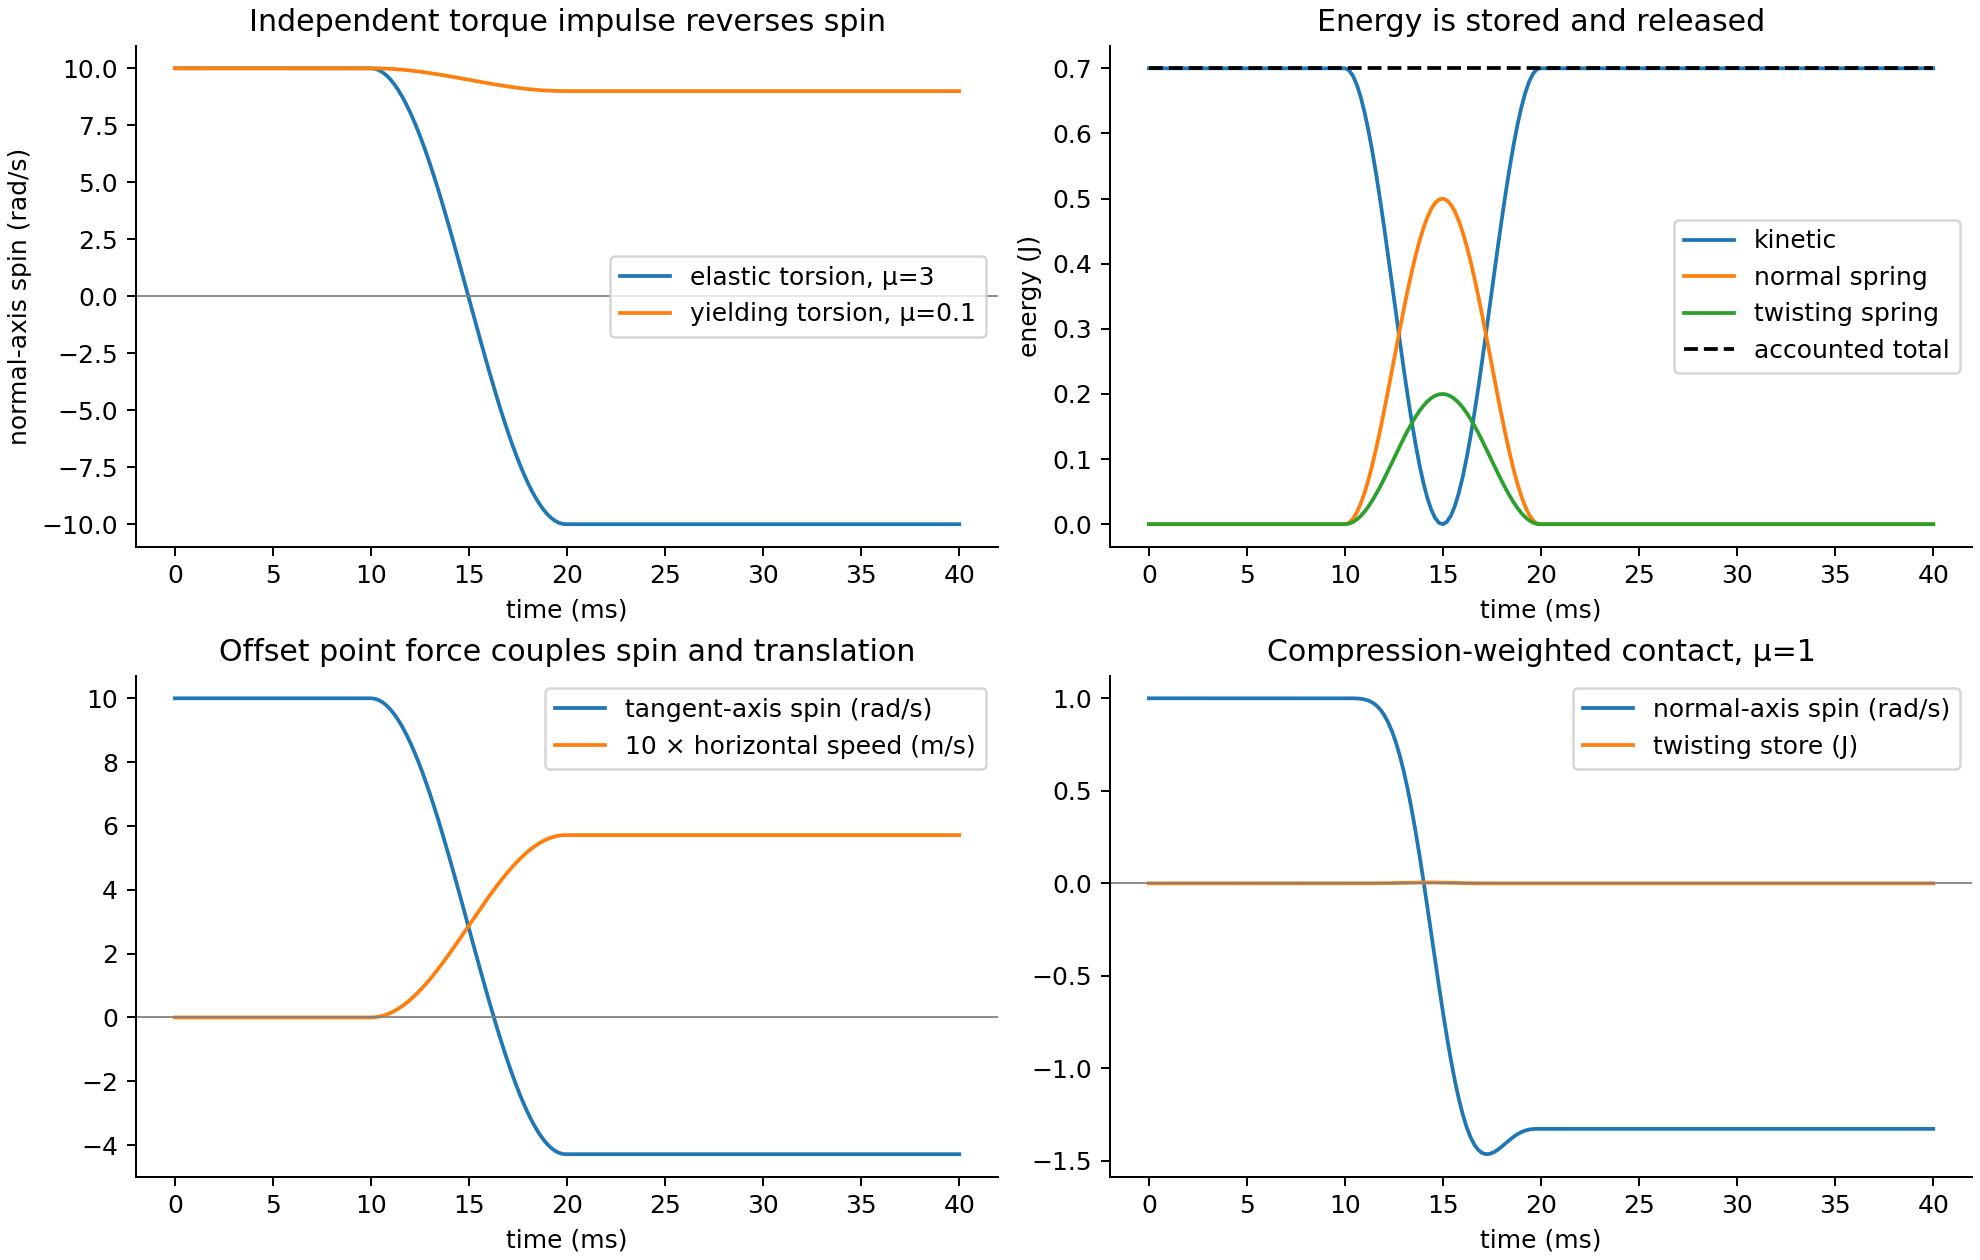
\includegraphics[width=\textwidth]{spin-energy.png}
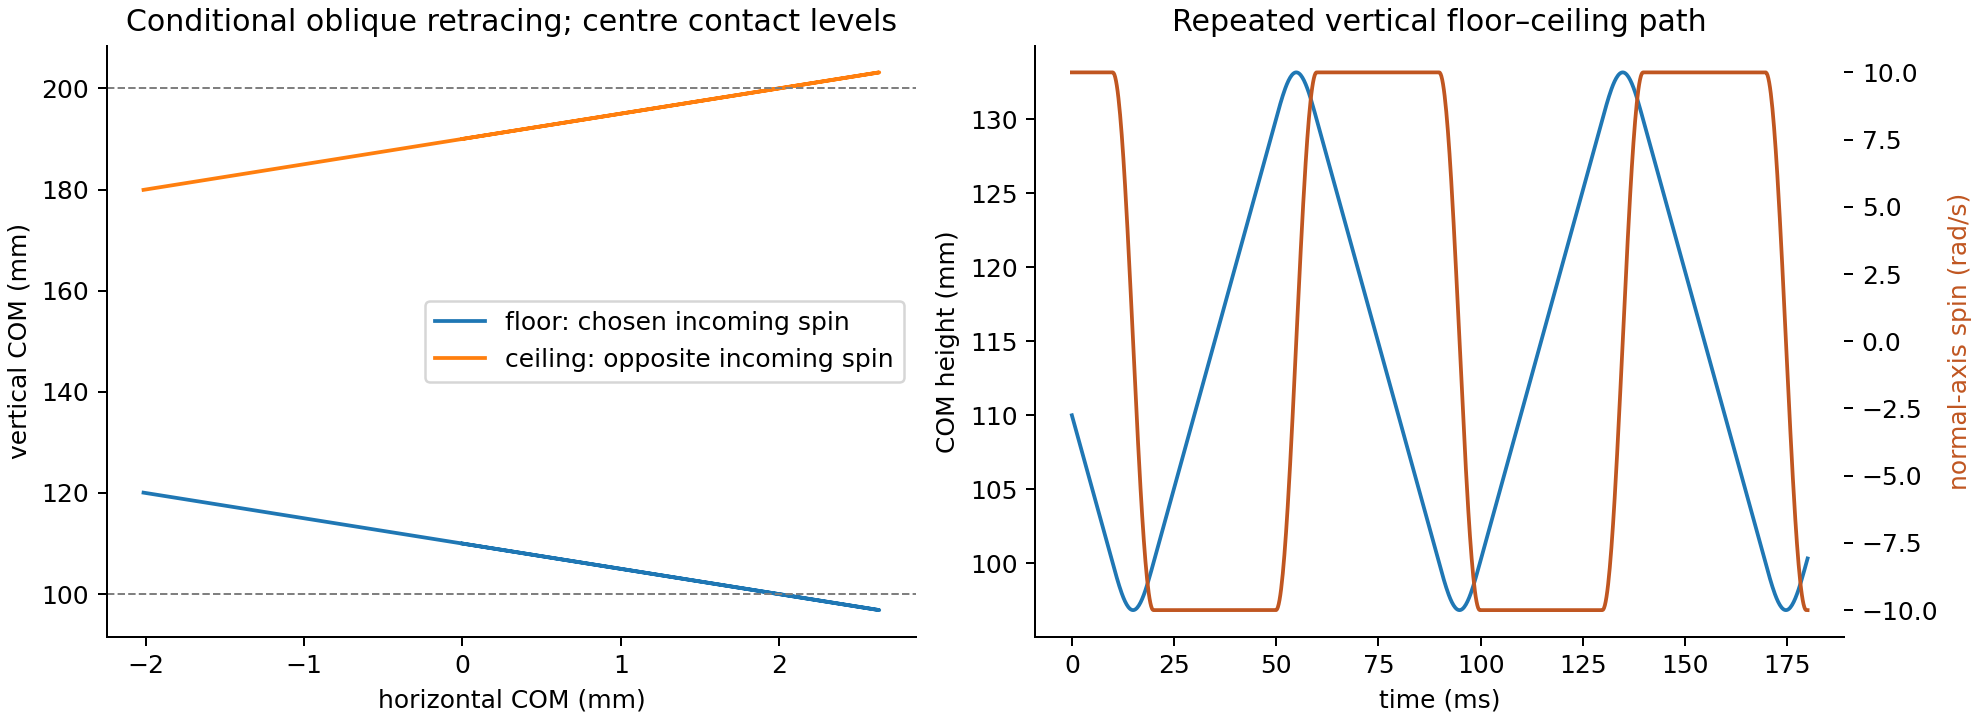
\includegraphics[width=\textwidth]{retrace.png}
\noindent
The weighted contact can transfer energy between normal and rotational channels, so a single-channel restitution may exceed one while total mechanics remain passive. Low friction can dissipate enough elastic input to prevent reversal. The same-material slow and rapid examples use speeds $0.01$ and $100$ m/s, demonstrating numerical behavior of this ideal law, not real rubber at those rates. All traces, failures, frozen parameters, source and three-level refinements are archived. This is a sphere/plane prototype; arbitrary-shape simultaneous contact needs separate engine validation. The accompanying literature review distinguishes known soft-finger mechanics from any unproven publication novelty.
\end{document}
